\documentclass[14pt]{extbook}
\usepackage{multicol, enumerate, enumitem, hyperref, color, soul, setspace, parskip, fancyhdr} %General Packages
\usepackage{amssymb, amsthm, amsmath, bbm, latexsym, units, mathtools} %Math Packages
\everymath{\displaystyle} %All math in Display Style
% Packages with additional options
\usepackage[headsep=0.5cm,headheight=12pt, left=1 in,right= 1 in,top= 1 in,bottom= 1 in]{geometry}
\usepackage[usenames,dvipsnames]{xcolor}
\usepackage{dashrule}  % Package to use the command below to create lines between items
\newcommand{\litem}[1]{\item#1\hspace*{-1cm}\rule{\textwidth}{0.4pt}}
\pagestyle{fancy}
\lhead{Makeup Progress Quiz -1}
\chead{}
\rhead{Version A}
\lfoot{7547-2949}
\cfoot{}
\rfoot{Fall 2020}
\begin{document}

\begin{enumerate}
\litem{
Describe the end behavior of the polynomial below.\[ f(x) = -9(x + 8)^{3}(x - 8)^{8}(x + 7)^{5}(x - 7)^{6} \]\begin{enumerate}[label=\Alph*.]
\begin{multicols}{2}\item 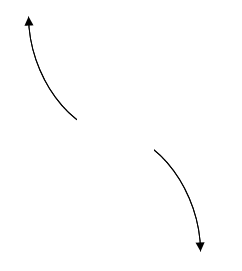
\includegraphics[width = 0.3\textwidth]{../Figures/polyEndBehaviorAA.png}\item 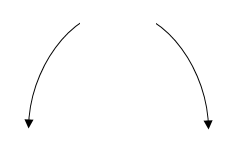
\includegraphics[width = 0.3\textwidth]{../Figures/polyEndBehaviorBA.png}\item 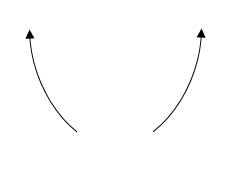
\includegraphics[width = 0.3\textwidth]{../Figures/polyEndBehaviorCA.png}\item 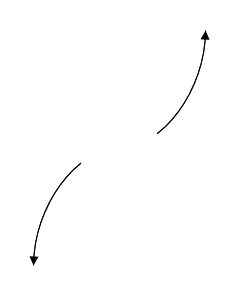
\includegraphics[width = 0.3\textwidth]{../Figures/polyEndBehaviorDA.png}\end{multicols}\item None of the above.
\end{enumerate} }
\litem{
Describe the zero behavior of the zero $x = 2$ of the polynomial below.\[ f(x) = 2(x + 4)^{7}(x - 4)^{6}(x - 2)^{10}(x + 2)^{7} \]\begin{enumerate}[label=\Alph*.]
\begin{multicols}{2}\item 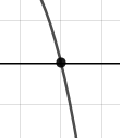
\includegraphics[width = 0.3\textwidth]{../Figures/polyZeroBehaviorCopyAA.png}\item 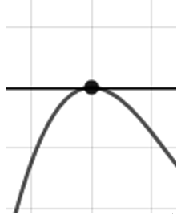
\includegraphics[width = 0.3\textwidth]{../Figures/polyZeroBehaviorCopyBA.png}\item 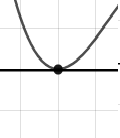
\includegraphics[width = 0.3\textwidth]{../Figures/polyZeroBehaviorCopyCA.png}\item 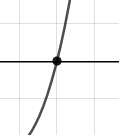
\includegraphics[width = 0.3\textwidth]{../Figures/polyZeroBehaviorCopyDA.png}\end{multicols}\item None of the above.
\end{enumerate} }
\litem{
Construct the lowest-degree polynomial given the zeros below. Then, choose the intervals that contain the coefficients of the polynomial in the form $x^3+bx^2+cx+d$.\[ -5 + 3 i \text{ and } -1 \]\begin{enumerate}[label=\Alph*.]
\item \( b \in [-3, 5], c \in [5, 16], \text{ and } d \in [-2, 9] \)
\item \( b \in [10, 15], c \in [39, 51], \text{ and } d \in [33, 40] \)
\item \( b \in [-3, 5], c \in [-2, 1], \text{ and } d \in [-11, -2] \)
\item \( b \in [-16, -7], c \in [39, 51], \text{ and } d \in [-42, -25] \)
\item \( \text{None of the above.} \)

\end{enumerate} }
\litem{
Describe the zero behavior of the zero $x = 8$ of the polynomial below.\[ f(x) = 6(x + 2)^{9}(x - 2)^{8}(x + 8)^{7}(x - 8)^{4} \]\begin{enumerate}[label=\Alph*.]
\begin{multicols}{2}\item 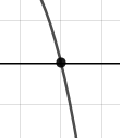
\includegraphics[width = 0.3\textwidth]{../Figures/polyZeroBehaviorAA.png}\item 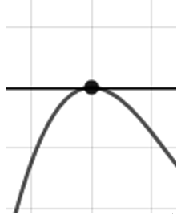
\includegraphics[width = 0.3\textwidth]{../Figures/polyZeroBehaviorBA.png}\item 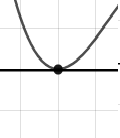
\includegraphics[width = 0.3\textwidth]{../Figures/polyZeroBehaviorCA.png}\item 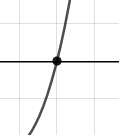
\includegraphics[width = 0.3\textwidth]{../Figures/polyZeroBehaviorDA.png}\end{multicols}\item None of the above.
\end{enumerate} }
\litem{
Which of the following equations \textit{could} be of the graph presented below?
\begin{center}
    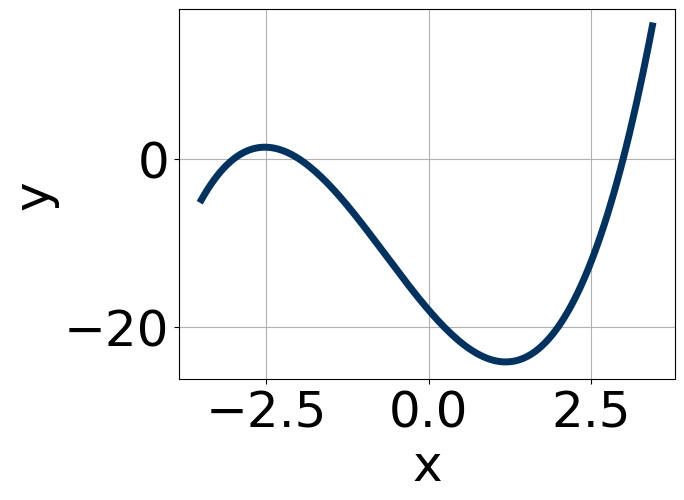
\includegraphics[width=0.5\textwidth]{../Figures/polyGraphToFunctionCopyA.png}
\end{center}
\begin{enumerate}[label=\Alph*.]
\item \( -20(x - 3)^{11} (x + 3)^{7} (x + 2)^{7} \)
\item \( 15(x - 3)^{4} (x + 3)^{11} (x + 2)^{7} \)
\item \( -4(x - 3)^{4} (x + 3)^{5} (x + 2)^{9} \)
\item \( 19(x - 3)^{10} (x + 3)^{8} (x + 2)^{5} \)
\item \( 13(x - 3)^{11} (x + 3)^{9} (x + 2)^{5} \)

\end{enumerate} }
\litem{
Which of the following equations \textit{could} be of the graph presented below?
\begin{center}
    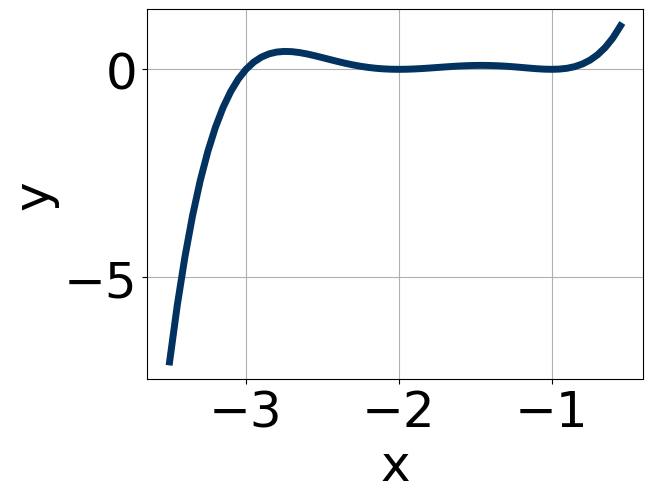
\includegraphics[width=0.5\textwidth]{../Figures/polyGraphToFunctionA.png}
\end{center}
\begin{enumerate}[label=\Alph*.]
\item \( 16(x + 1)^{10} (x + 2)^{8} (x + 3)^{9} \)
\item \( 11(x + 1)^{4} (x + 2)^{11} (x + 3)^{7} \)
\item \( -3(x + 1)^{10} (x + 2)^{4} (x + 3)^{4} \)
\item \( -16(x + 1)^{6} (x + 2)^{6} (x + 3)^{11} \)
\item \( 12(x + 1)^{8} (x + 2)^{11} (x + 3)^{4} \)

\end{enumerate} }
\litem{
Describe the end behavior of the polynomial below.\[ f(x) = 9(x + 4)^{2}(x - 4)^{5}(x + 8)^{3}(x - 8)^{4} \]\begin{enumerate}[label=\Alph*.]
\begin{multicols}{2}\item 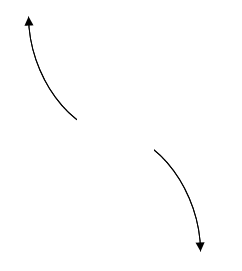
\includegraphics[width = 0.3\textwidth]{../Figures/polyEndBehaviorCopyAA.png}\item 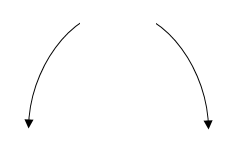
\includegraphics[width = 0.3\textwidth]{../Figures/polyEndBehaviorCopyBA.png}\item 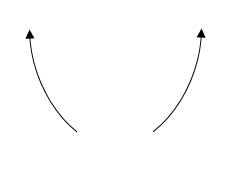
\includegraphics[width = 0.3\textwidth]{../Figures/polyEndBehaviorCopyCA.png}\item 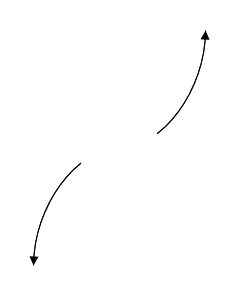
\includegraphics[width = 0.3\textwidth]{../Figures/polyEndBehaviorCopyDA.png}\end{multicols}\item None of the above.
\end{enumerate} }
\litem{
Construct the lowest-degree polynomial given the zeros below. Then, choose the intervals that contain the coefficients of the polynomial in the form $ax^3+bx^2+cx+d$.\[ \frac{1}{2}, -5, \text{ and } \frac{-3}{4} \]\begin{enumerate}[label=\Alph*.]
\item \( a \in [1, 9], b \in [50, 52], c \in [46, 55], \text{ and } d \in [12, 18] \)
\item \( a \in [1, 9], b \in [35, 44], c \in [6, 12], \text{ and } d \in [12, 18] \)
\item \( a \in [1, 9], b \in [-32, -28], c \in [-48, -38], \text{ and } d \in [-16, -13] \)
\item \( a \in [1, 9], b \in [35, 44], c \in [6, 12], \text{ and } d \in [-16, -13] \)
\item \( a \in [1, 9], b \in [-50, -37], c \in [6, 12], \text{ and } d \in [12, 18] \)

\end{enumerate} }
\litem{
Construct the lowest-degree polynomial given the zeros below. Then, choose the intervals that contain the coefficients of the polynomial in the form $x^3+bx^2+cx+d$.\[ 3 - 3 i \text{ and } 4 \]\begin{enumerate}[label=\Alph*.]
\item \( b \in [8, 14], c \in [39, 42.7], \text{ and } d \in [66, 81] \)
\item \( b \in [-11, -7], c \in [39, 42.7], \text{ and } d \in [-75, -67] \)
\item \( b \in [-8, 2], c \in [-7.7, -5.8], \text{ and } d \in [12, 17] \)
\item \( b \in [-8, 2], c \in [-2.9, 0.2], \text{ and } d \in [-19, -11] \)
\item \( \text{None of the above.} \)

\end{enumerate} }
\litem{
Construct the lowest-degree polynomial given the zeros below. Then, choose the intervals that contain the coefficients of the polynomial in the form $ax^3+bx^2+cx+d$.\[ 5, \frac{6}{5}, \text{ and } 1 \]\begin{enumerate}[label=\Alph*.]
\item \( a \in [-2, 6], b \in [-37, -32], c \in [56, 63], \text{ and } d \in [-34, -28] \)
\item \( a \in [-2, 6], b \in [-37, -32], c \in [56, 63], \text{ and } d \in [29, 33] \)
\item \( a \in [-2, 6], b \in [8, 19], c \in [-51, -45], \text{ and } d \in [29, 33] \)
\item \( a \in [-2, 6], b \in [35, 40], c \in [56, 63], \text{ and } d \in [29, 33] \)
\item \( a \in [-2, 6], b \in [22, 27], c \in [-9, 0], \text{ and } d \in [-34, -28] \)

\end{enumerate} }
\end{enumerate}

\end{document}